\setchapterpreamble[or][.5\textwidth]{%
\dictum[ Joseph Weizenbaum]{%
A computer will do what you tell it to do, but that may be much different from what you had in mind.}\vskip1em}


\chapter{Finite element based discretization}
\label{NumericalSolution}
%\epigraphhead[5]{\epigraph{ A computer will do what you tell it to do, but that may be much different from what you had in mind.}{ Joseph Weizenbaum}}

Unfortunately the boundary value problem (BVP) of elasticity can (with exception of a few simple cases) not be solved analytically. In this chapter, we outline a numerical approach for solving the linear BVP (\ref{LinearElasticityFormulation}) based on the finite element method (FEM). It should be pointed out that the approach generalizes very well to the non-linear problem.

\section{Getting Started}

The core idea of the FE method is to determine the exact solution for the BVP not in a continuous (infinite-dimensional) space $V$, but rather in the discrete (finite-dimensional) sub-space $V_h \subset V$. In order to achieve that goal the partial differential equations of the BVP are transformed into a so called weak formulation. The weak formulation only requires the solution to hold only with respect to so called test functions. Although this concept seems odd at first (and much more complicated than the original partial differential equations), we will quickly see that it can be discretized very elegantly. We will also discover that the weak formulation is identical with the minimization of certain energy functionals (variational formulation). Especially in the static case this opens up a very vivid physical interpretation of the formulation (minimum of the energy stored in the elastic system). It is subsequently shown how the variational form can be discretized into a system of linear ordinary differential equations (more information cane be found in the appendix). Two important time integration techniques that can be used to solve those ODEs are presented in section \ref{TimeIntegration}. Finally, a very efficient FE formulation based on quadratic tetrahedral elements for real-time applications is detailed.

\section{Variational formulation}

\subsection{Weak solution in Sobolev spaces}

\label{SubSectionWeakSolutions}
The basic idea of a finite element method is to discretize the physical problem in a so called weak (or variational) form instead of its classical strong formulation. For this purpose we define the test functions $\mTFunc \in \mSCTFunc$ with compact support that vanish on the Dirichlet boundary $\mBCD$. Then, we demand that the $L^2$ scalar product 

 \begin{equation}
\mIntRConf \left( \mDiv \msigma +    \rho _0 \mbg  -  \rho _0 \ddot \mbu \right) \mTFunc \mDRConf = 0 \qquad \forall \mTFunc
\label{WeakFormulationRaw}
\end{equation}

between the residual of the partial differential equation (PDE) and the test functions vanishes for all $\mTFunc$. Rephrasing the divergence term using the product differentiation rule


 \begin{equation}
 \mDiv \msigma \cdot \mTFunc = \mDiv ( \msigma  \mTFunc) - \msigma : \mGrad \mTFunc
\end{equation}

and application of the divergence theorem yields
\begin{eqnarray}
\mIntRConf   \mDiv \msigma \cdot \mTFunc \mDRConf &=& \mIntRConf \mDiv ( \msigma  \mTFunc) \mDRConf  - \mIntRConf   \msigma : \mGrad \mTFunc \mDRConf \\
&=& \int _{\mBCN}  \mt \cdot \mTFunc \mbdAZero  - \mIntRConf  \msigma : \mGrad \mTFunc \mDRConf.
\label{ApplicationsDivTheorem}
\end{eqnarray}

Here, $\mt$ are the prescribed traction boundary conditions on $\mBCN$. Inserting this in eq. \ref{WeakFormulationRaw} gives rise to the weak form of Cauchy's equation of motion:
\begin{equation}
\mIntRConf \msigma : \mGrad \mTFunc\mDRConf - \int _{\mBCN}  \mt \cdot \mTFunc \mbdAZero - \mIntRConf \left( \rho _0 \mbg  \cdot \mTFunc  +  \rho _0 \ddot {\mbu} \cdot \mTFunc \right) \mDRConf = 0.
\label{WeakFormulation}
\end{equation}

It is apparent, that each $\mbu$ which solves the original boundary value problem (BVP) is also a solution to the weak formulation. It can also be shown that each $\mbu \in \mSSolBC$ for which eq. (\ref{WeakFormulation}) holds is also a solution of the classical PDE \cite{Braess2007}. However, if we only assume $\mbu \in \mBCSPD \cap \mBCSPN$ and not $\mbu \in \mSSol$, then the weak formulation has more solutions than the classical one. Through the definition of weak derivatives the space of all solutions $\mbu \in  \mBCSPD \cap \mBCSPN$ to eq. \ref{WeakFormulation} can be identified with the Sobolev space $H^1(\Omega)$ \cite{Braess2007}. It should be noted that there are physical problems (e.g. shock problems) which have no classical solutions, but do have a solution in $H^1(\Omega)$. 

The solution space is not only a Sobolev space, but also a Hilbert space (hence the notation $H^1(\Omega)$).  Thus, the powerful tools of functional analysis open up a natural way of discretizing the weak form by finite element based techniques. Also, the concept of weak solutions in Sobolev spaces is a very useful tool in the analysis of uniqueness and existence of solutions to BVP. In particular, the Lax-Milgram theorem establishes that the bilinear form (\ref{WeakFormulationRaw}) has a unique solution if it is strongly coercive \cite{Braess2007}.


\subsection{Static formulation: Minimizing energy functionals}

In the following section we will formulate the static problem in terms of minimizing the total energy of $\mBody$. It will become apparent that this variational formulation is identical to the weak formulation. This physics-based derivation provides an elegant and intuitive access to weak formulations and will be extensively used in this thesis. 

The total potential energy of the system can be formally derived from the balance of mechanical energy for linear elasticity eq. (\ref{MechEnergyBalanceLinear}). For this purpose we assume that each particle in $\mBody$ is at rest at the beginning of the simulation, i.e. $\mv(\mbx,t=0)=0$. Omitting the inertia forces (static approximation) and integrating eq. (\ref{MechEnergyBalanceLinear}) over time then yields
 \begin{equation}
 \meFunc(\mbu) =     \mIntRConf \msigma : \meps  \mdVZero      -  \mIntBCRConf \mt \cdot \mbu   \mbdAZero  -  \mIntRConf \rho \mbg \cdot \mbu \mdVZero.
\label{MechEnergyStaticLinear}
\end{equation}

The solution to the static problem can be interpreted as the configuration that minimizes this energy functional.  The principle of stationary potential energy states a necessary condition for a stationary point in $\meFunc(\mbu)$: It requires the directional derivative with respect to the displacements $\mbu$ 
 \begin{equation}
 \meFunc(\mbu, \delta \mbu) = D_{\delta \mbu} \meFunc (\mbu) = \left. \frac{\textnormal{d}}{\textnormal{dh}} \meFunc (\mbu + h \delta \mbu) \right| _{h=0} = 0
\end{equation}
to vanish in all directions \cite{Holzapfel2000}. Carrying out the variation on the internal elastic energy yields:

 \begin{alignat}{1}
D_{\delta \mbu} \meFunc (\mbu) _{int} &= \left. \frac{\textnormal{d}}{\textnormal{dh}} \mIntRConf \msigma : \meps  \mdVZero \right| _{h=0}   \\
&= \left. \frac{\textnormal{d}}{\textnormal{dh}} \mIntRConf \msigma : \frac{1}{2}((\nabla \mbu + h \nabla \delta \mbu) +(\nabla \mbu + h \nabla \delta \mbu)^T) \mdVZero \right| _{h=0} \\
&= \left. \mIntRConf \msigma : \frac{1}{2}( \delta \nabla \mbu + \delta \nabla \mbu^T) \mdVZero \right| _{h=0}  \\
&=  \mIntRConf \msigma : \delta \frac{1}{2} ( \nabla \mbu + \nabla \mbu^T) \mdVZero  =   \mIntRConf \msigma : \delta \meps  \mdVZero 
\label{InternalVariations}
\end{alignat}

Similarly, the external energies (loads) can be expressed as
 \begin{alignat}{1}
D_{\delta \mbu} \meFunc (\mbu) _{ext} &= \left. \frac{\textnormal{d}}{\textnormal{dh}} \mIntBCRConf \mt \cdot (\mbu + h \delta \mbu)   \mdAZero +  \frac{\textnormal{d}}{\textnormal{dh}} \mIntRConf \rho \mbg \cdot (\mbu + h \delta \mbu) \mdVZero \right| _{h=0}   \\
&= \mIntBCRConf \mt \cdot \delta \mbu   \mdAZero  +  \mIntRConf \rho \mbg \cdot \delta \mbu \mdVZero
\label{ExternalVariations}
\end{alignat}

and thus the complete variational form is
 \begin{alignat}{1}
& D_{\delta \mbu} \meFunc (\mbu) = D_{\delta \mbu} \meFunc (\mbu)_{int} + D_{\delta \mbu} \meFunc (\mbu)_{ext}  = 0 \\
\Leftrightarrow \qquad & \mIntRConf \msigma : \delta \meps  \mdVZero = \mIntBCRConf \mt \cdot \delta \mbu   \mdAZero  +  \mIntRConf \rho \mbg \cdot \delta \mbu \mdVZero.
\label{VariationalFormStatic}
\end{alignat}

We can thus summarize the variational formulation of the static elasticity problem: Find the displacement field $\mbu \in V = {H^1(\Omega) \cap \mBCSPD \cap \mBCSPN}$, s.t. eq. (\ref{VariationalFormStatic}) holds for all $\mTFunc \in \mSCTFuncThree$. It can be quickly shown (symmetry of $\msigma$) that the variational form is equivalent to the weak formulation. 

\subsection{Dynamic formulation: Hamiltonian variational principle}

In the dynamic case, the intuitive formulation in terms of minimizing the elastic energy is replaced by the principle of least action \cite{Ibrahimbegovic2009}. More formally we now seek the stationary point of the Hamiltonian variational principle.

With the same assumptions that we made in the static case, we can derive the Lagrangian

 \begin{alignat}{1}
\mL(\mbu) &=  \meFunc(\mbu) - \mK (\dot{\mbu}) \\
&= \mIntRConf \msigma : \meps  \mdVZero      -  \mIntBCRConf \mt \cdot \mbu   \mbdAZero  -  \mIntRConf \rho \mbg \cdot \mbu \mdVZero - \mIntRConf \frac{1}{2} \rho_0  {\dot \mbu} ^2 \mdVZero
\label{MechEnergyDynamicLinear}
\end{alignat}

of the system \cite{Holzapfel2001}. The solution to the dynamic elasticity problem can then be regarded as a stationary point of the Hamiltonian variational principle
 \begin{alignat}{1}
& D_{\delta \mbu} \mH (\mbu) = \int _0 ^T \mL (\mbu) \mintdt
%& = \int _0 ^T \left\{ \mIntRConf \rho \ddot{\mbu}  \delta \mbu \mdVZero   + \mIntRConf \msigma : \delta \meps  \mdVZero = \mIntBCRConf \mt \cdot \delta \mbu   \mdAZero  +  \mIntRConf \rho \mbg \cdot \delta \mbu \mdVZero \right\}dt
\label{HamiltonianVariationalForm}
\end{alignat}



We compute the variation of the kinetic part of the Hamiltonian using integration by parts:
 \begin{alignat}{1}
&D_{\delta \mbu} \mH_{kin} (\mbu)  = \left. \frac{\textnormal{d}}{\textnormal{dh}} \int _0 ^T - \mIntRConf \frac{1}{2} \rho_0  (\frac{\textnormal{d}( \mbu  + h \delta \mbu)}{\textnormal{dt}} ) ^2 \mdVZero \mintdt  \right| _{h=0} \\
&= \left.  - \mIntRConf \int _0 ^T \frac{1}{2} \rho_0  2 \frac{\textnormal{d}( \mbu  + h \delta \mbu)}{\textnormal{dt}} \frac{\textnormal{d}}{\textnormal{dh}} \frac{\textnormal{d}( \mbu  + h \delta \mbu)}{\textnormal{dt}}   \mintdt \mdVZero \right| _{h=0}  \\
&=  \left.   \mIntRConf \left( - \left[  \rho_0  \frac{\textnormal{d}( \mbu  + h \delta \mbu)}{\textnormal{dt}} \delta \mbu   \right]_0 ^T  +  \int _0 ^T \rho_0   \frac{\textnormal{d}^2( \mbu  + h \delta \mbu)}{\textnormal{dt}^2} \delta \mbu  \mintdt  \right) \mdVZero  \right| _{h=0} \\
&=    \mIntRConf \left( -  \rho_0  \frac{\textnormal{d} \mbu }{\textnormal{dt}} \delta \underbrace{\mbu(T)}_{=0} + \rho_0  \frac{\textnormal{d} \mbu }{\textnormal{dt}} \delta \underbrace{\mbu(0)}_{=0}  +  \int _0 ^T \rho_0   \frac{\textnormal{d}^2 \mbu }{\textnormal{dt}^2} \delta \mbu  \mintdt  \right) \mdVZero  \\
&=   \int _0 ^T \mIntRConf  \rho_0   \ddot \mbu \delta \mbu    \mdVZero  \mintdt
\label{KineticVariations}
\end{alignat}

The final result was obtained by imposing that the variations are zero at both limits of the time interval. By using the previous results obtained in the static case eq. (\ref{VariationalFormStatic}), the complete variation of the Hamiltonian reads

 \begin{alignat}{1}
&D_{\delta \mbu} \mH (\mbu)  =  \\
& \int _0 ^T \left( \mIntRConf  \rho_0   \ddot \mbu \delta \mbu    \mdVZero  + \msigma : \delta \meps  \mdVZero - \mIntBCRConf \mt \cdot \delta \mbu   \mdAZero -  \mIntRConf \rho \mbg \cdot \delta \mbu \mdVZero \right)\mintdt.
\label{CompleteHamiltonianVariation}
\end{alignat}

It is reasonable to require the above equation to hold for all T during the simulation. Thus, the dynamic problem can be posed in its corresponding time-differential, space variational form: Find the displacement field $\mbu \in  V = {H^1(\Omega) \cap \mBCSPD \cap \mBCSPN}$, s.t. 
 \begin{alignat}{1}
 \mIntRConf  \rho_0   \ddot \mbu \delta \mbu    \mdVZero  + \mIntRConf  \msigma : \delta \meps  \mdVZero - \mIntBCRConf \mt \cdot \delta \mbu   \mdAZero  -  \mIntRConf \rho \mbg \cdot \delta \mbu \mdVZero = 0
\label{DynamicVariationalForm}
\end{alignat}
holds for all $\mTFunc \in \mSCTFuncThree$. 




\section{Finite element discretization}
\label{FEDiscretizationSection}
The idea of the finite element discretization technique is to not look for a solution $\mbu$ to the variational problem in the infinite-dimensional space $V$ of continuous functions, but to an approximated solution $\mbu _h$ in a suitable finite-dimensional, discrete sub-space $V_h \subset V$. This subspace is typically spanned by piecewise continuous polynomial functions that have \emph{small} support. In order to define these function spaces, $\Omega$ is divided into different polyhedral elements (Fig. \ref{FEDiscretization}). In this context the boundary of $\Omega$ is required to be sufficiently smoothed which is formalized through the assumption that $\Omega$ is a Lipschitz domain. 

When constructing the finite element space we are facing the fundamental problem that is associated with every discretization technique: How to find the best approximation to the correct solution with a given amount of complexity in terms of degrees of freedom of the discrete system. An important reason for the success of the FE-method are the powerful and elegant tools that are available for a-priori error approximation. At the core, C\'{e}a's lemma states that the finite element approximation $\mbu_h$ is the near best fit to the solution $\mbu$ in the norm associated with $H^1$ \cite{Braess2007}. Geometrically speaking, the discrete solution $\mbu_h$ is the orthogonal projection of $\mbu$ into $V_h$ with respect to the inner product that is induced by the bilinear form (\ref{WeakFormulationRaw}). It follows that the construction of the subspace $V_h$ is crucial for the accuracy of the method.

The convergence of FE methods is typically studied in suitable mesh-dependent norms. Thus, several a-priori error estimates exist for different norms and different finite element types. For finite element spaces that are spanned by piecewise polynomials of order $p$ on tetrahedral and hexahedral elements, it can be shown that the convergence rate for is of order $p+1$ if the real solution is sufficiently smooth. However, the latter is usually not the case in many applications. Thus first or second order polynomials are typically used for elasticity problems.

\begin{figure}
   \centering   
   \psfragfig[width=0.7\textwidth]{Figures/FEDiscretization}
	\caption{A two dimensional body $\mathcal B$ (grey line) is discretized with a triangular finite element mesh $\mathcal M$ (dashed lines). The set of vertices $\mVertSetElem_I$ that form the element $\mElem_I$ is shown in green, while the set of all elements $\mElemSetVert_I$ around the vertex $\mVert_I$ is colored blue.}
\label{FEDiscretization}
\end{figure}

A finite element mesh $\mMesh$ with elements $\mElem_I$ and $n$ vertices $\mVert_I$ is defined to support the basis functions that span the solution space $V_h$. We denote the set of all elements $\mElem_J$ around the vertex $\mVert_I$ with $\mElemSetVert_I$. Similarly $\mVertSetElem_I$ is the set of vertices that form the element $\mElem_I$. Typically so called nodal basis functions $\mbf$ are used. Each nodal functions $\mbf$ satisfies
\begin{equation}
\mbf(\mVert_I) = \delta _{IJ}  
\label{DeltaProperty}
\end{equation}

i.e. it is zero at every other node except the associated $J$-th node ($\delta$-property). Furthermore, the nodal basis function satisfy the \emph{partition of unity} 
\begin{equation}
\sum _{J \in \mVertSetElem_I } \mbf(\mbx) = 1 \quad \forall \mbx \in \mElem_I
\label{PartitionOfUnity}
\end{equation}

and have a \emph{small}, compact support, i.e.
\begin{equation}
 \mbf(\mbx) = 0 \quad \forall \mbx \notin \mElemSetVert_J.
\end{equation}

The nodal basis functions for linear and quadratic tetrahedral elements can be found in appendix \ref{AShapeFunctions}. In order to discretize the weak formulation, $\mbu_h$ is expressed by the linear combination
\begin{equation}
\mbu_h (t) = \mbu_h  = \sum _{J=1} ^\mnnode \mcu_J   \mbf  =   \mcu_J  \mbf =  \mcu_{jJ}   \mbffull 
\label{FEInterpolation}
\end{equation}

of the $\mnnode$ basis functions $\mbf$ with the time dependent coefficients $\mcu $ or $\mcu (t)$ (in the above equation and from here on out summation over repeated indices is implied). As a direct consequence of the $\delta$-property, the coefficients $\mcu (t)$ coincide with the displacements of the element nodes when using nodal basis functions. Due to the special form of the basis functions, the solution $\mbu_h$ is $C^0$-continuous and we have $V_h \subset V$. It is only through this so called conformal finite element space that statements on uniqueness and existence of solutions can be directly transferred from the continuous to the discrete problem.

For later use, we also introduce the displacement gradient 
\begin{equation}
\nabla \mbu  = \nabla (\mcu_J  \mbf ) = \mcu_J \nabla \mbf.
\label{DiscreteDispGradient}
\end{equation}


It is theoretically possible to use different function spaces for $\mbu _h$ and the test functions $\delta \mbu _h$. However, in practice we usually choose these spaces to be the same (Galerkin method). Thus we have
\begin{equation}
\delta \mbu = \sum _{I=1} ^\mnnode \delta \mcu_I \mtf  =  \delta \mcu_I \mtf
\end{equation}

\subsection{Matrix formulation}
\label{SectionMatrixFormulation}

By inserting the basis functions and the test functions into the variational formulation (\ref{DynamicVariationalForm}) and performing numerical integration, a linear system of ordinary differential equations can be derived. In the following we sketch this procedure and derive the load vector as well as the mass and the stiffness matrix.

We start by inserting the test functions into the expression for the external forces eq. (\ref{ExternalVariations}) to derive 
\begin{alignat}{1}
D_{\delta \mcu} \meFunc (\mbu _h) _{ext} &= \mIntBCRConf \mt \cdot \left( \delta \mcu _I \mtf \right)  \mdAZero  +  \mIntRConf \rho g \cdot \left( \delta \mcu _I \mtf \right) \mdVZero \\
&= \delta \mcu _I \left( \mIntBCRConf \mt \cdot  \mtf   \mdAZero  +  \mIntRConf \rho g \cdot \mtf \mdVZero  \right)  = \delta \mcu _I \mfextTwo.
\label{fext}
\end{alignat}

As the test functions are polynomials, the surface and volume integrals in (\ref{fext}) can be accurately and efficiently evaluated using numerical integration techniques such as Gaussian quadrature. For an overview on this topic we refer to Zienkiewicz et al. \cite{Zienkiewicz1977}. The resulting external load vector $\mfextTwo$ (sometimes also written as $\mfext$ or $\mfextThree$) denotes the force that acts on each node $\mnode_I$ in the spatial direction $j$. Its length is thus $3 \mnnode$.

Similarly, the discretization of the inertia forces (variation of kinetic energy) (\ref{KineticVariations}) yields
\begin{alignat}{1}
D_{\delta \mcu} \meFunc (\mbu _h) _{kin} &= \mIntRConf \rho \left( \ddot{\mcu}_J \mbf  \right)  \left( \delta \mcu _I \mtf \right)  \mdVZero =  \delta \mcu _I \mIntRConf \rho \mbf \ddot{\mcu}_J    \mtf \mdVZero \\
&=  \delta \mcu_I \left( \mIntRConf \rho \mbf  \mtf \mdVZero \right) \ddot{\mcu}_J = \delta \mcu _I \mmmat_{IJ} \ddot{\mcu}_J.
\label{MassMatrix}
\end{alignat}
The entries of the so called mass matrix $\mmmat_{IJ}$ (sometimes also denoted with $\mmmat$ or $\mmmat_{iIjJ}$) are again computed using numerical integration. The vector $\ddot{\mcu}_J$ (or simply $\ddot{\mcu}$) is the vector of nodal accelerations. 

The internal forces obviously depend on the deformation field $\mbu_h$ and thus on the vector of nodal displacement $\mcu$ (i.e. the coefficients of the basis functions). If the displacement is known we can compute the internal nodal forces using numerical integration. Due to the symmetry of $\msigma$ we can derive:
\begin{alignat}{1}
D_{\delta \mcu} \meFunc (\mbu _h) _{int} &= \mIntRConf \msigma : \delta \meps  \mdVZero =  \mIntRConf \msigma : \frac{1}{2} \left( \delta \nabla \mbu + (\delta \nabla \mbu)^T \right)  \mdVZero \\
&=  \mIntRConf \msigma :  \delta \nabla \mbu  \mdVZero = \mIntRConf \msigma : \left( \delta \mcu_I \nabla \mtf \right) \mdVZero \\
&= \delta \mcu_{iI} \mIntRConf \msigma_{ik}  (\nabla \mtfTwo)_{kI} \mdVZero = \delta \mcu_{iI} \mIntRConf  \mfintDens \mdVZero\\
&= \delta \mcu_{iI} \mfintThree = \delta \mcu_I \mfintTwo 
\label{fint}
\end{alignat}

Here, $\mfintDens$ denotes internal force density. For implicit integration schemes or non-linear static solvers of Newton-Raphson type, the tangent stiffness matrix 
\begin{alignat}{1}
\msmat _{IJ} = K _{iIjJ} = \frac{\partial \mfintThree}{\partial \mcu_{jJ}} = \mIntRConf \frac{\partial \mfintDens}{\partial \mcu_{jJ}} \mdVZero = \sum_{\mElem} \mIntREl \frac{\partial \mfintDens}{\partial \mcu_{jJ}} \mdVZero = \sum_{\mElem} \mathbf{K}^{\mElem}
\label{StiffnessMat}
\end{alignat}
is necessary. From the above equation it is apparent how the global stiffness matrix $\msmat _{IJ}$ is constructed: First, the integrals in the above equation are evaluated on a per-element basis. Due to the small support of the basis functions, only few integrals (e.g. 12 for the linear tetrahedron) have to be evaluated for each row. These elemental matrices $\mathbf{K}^{\mElem}$ are then added into the global data structure (\emph{matrix assembly}).

For the linear elastic model, the entries of the tangent stiffness matrix can be computed as (please refer to the appendix \ref{ANodalForces} for details):
\begin{alignat}{1}
K _{iIjJ} = \mIntRConf \left( \mu \nabla \mtfn_{iJ} \nabla \mtfn_{jI} + \mu \delta_{IJ} \sum_{l=1} ^3 \nabla \mtfn_{il} \nabla \mtfn_{jl} +\lambda \nabla \mtfn_{iI} \nabla \mtfn_{jJ}  \right)\mdVZero
\end{alignat}

Here, $\delta_{IJ}$ again denotes the Kronecker-delta symbol and $\mu, \lambda$ are the material parameters. For linear elasticity, there is
\begin{equation}
\mfint = \msmat_{IJ} \mcu_{J}.
\label{FintStiffnessMat}
\end{equation}

The global matrices $\mmmat, \msmat$ are symmetric, positive definite sparse matrices. Their sparsity pattern depends on the mesh topology and is thus is irregular for unstructured grids. 

Using the obtained discretization of the external, inertia and internal forces we can state the discrete variational form

 \begin{alignat}{1}
 D_{\delta \mbu} \meFunc (\mbu)_{kin} + D_{\delta \mbu} \meFunc (\mbu)_{int} &= D_{\delta \mbu} \meFunc (\mbu)_{ext}  \\
 \Leftrightarrow \qquad \qquad \delta \mcu _I \mmmat_{IJ} \ddot{\mcu}_J + \delta \mcu_I \mfint &= \delta \mcu _I \mfextTwo
\end{alignat}

As the equation holds for all variations $\delta \mcu_I$, the variational form can be stated as a system of second order ordinary differential equations (ODE):

 \begin{eqnarray}
\mmmat \ddot{\mcu} +  \mfint = \mfext  
\label{DisEquationOfMotion}
\end{eqnarray}

This equality also holds for non-linear problems. For the linear elastic formulation, the internal nodal forces depend linearly on the nodal displacements eq. (\ref{FintStiffnessMat}) and we can express the equilibrium equations through the following system of linear second order ODE's:

 \begin{alignat}{1}
\mmmat \ddot{\mcu} +  \msmat \mcu = \mfext
\label{LinMatEquationOfMotion}
\end{alignat}

Neumann boundary conditions (forces on the surface) are reflected in the formulation through the external forces $\mfext$. In the following section, we will see how Dirichlet boundary conditions (prescribed displacements) can be imposed during the linear system solve once the system of ODEs has been discretized using time integration techniques.


\section{Time integration}
\label{TimeIntegration}
In this section we derive the full discretization, i.e. we discretize the ODEs in time to derive a linear system of equations. The methods are presented with linear elasticity in mind, but easily generalize to non-linear problems. 

For viscoelastic models the internal nodal forces also encapsulate the viscoelastic behavior (see section \ref{Viscoelasticity}). Consequently, we can define the tangent damping matrix
\begin{eqnarray}
\mdmat _{IJ} = D _{iIjJ} = \frac{\partial \mfintThree}{\partial \dot{\mcu}_{jJ}}
\label{DampingMat}
\end{eqnarray}
in addition to the tangent stiffness matrix eq. (\ref{FintStiffnessMat}). Time integration methods can be categorized into explicit and implicit methods. The explicit methods enforce the equilibrium (\ref{DisEquationOfMotion}) only at the beginning of the time step at the current time $t$, whereas implicit algorithms enforce it at the end of the time step at time $t+\mdt$ ($\mdt$ is the time step size). Explicit methods are very computationally efficient, as their computation only require matrix-vector operations. In contrast, implicit methods require solving a system of equations for every time step. However, explicit methods are only conditionally stable. Especially for stiff systems, they need very small timesteps to remain stable. Thus they are often a poor choice for soft tissue simulations especially for nearly incompressible material models \cite{Sueli2003}. For real-time deformable model problems, implicit methods have emerged as the dominant means for time discretization \cite{Baraff1998}.

In the following, we describe the dynamic equilibrium (\ref{DisEquationOfMotion}) at time $t+\mdt$ under the assumption that the system is in equilibrium at time $t$. From now on we denote the point in time for each nodal quantity with left superscript (e.g. $t+\mdt$). The superscript $t$ which indicates the current time is omitted when apparent from the context. We also define
\begin{equation}
\mcdu = \mtvh \mcu - \mth \mcu   \qquad \textnormal{and} \qquad \mcdv = \mtvh \mcv - \mth \mcv.
\end{equation}

Using the tangent stiffness matrix and the tangent damping matrix, we can express the first order Taylor expansion of $\mfint$ around $t$ as
\begin{eqnarray}
\mtvh \mfint &=& \mth \mfint + \frac{\partial \mfint}{\partial {\mcv}} (\mtvh \mcv - \mth \mcv) + \frac{\partial \mfint}{\partial {\mcu}} (\mtvh \mcu - \mth \mcu) \\
&=& \mth \mfint + \mdmat \dot{\mcdu} + \msmat \mcdu.
\end{eqnarray}

As the external forces (\emph{dead loads}) do not depend on the deformation, i.e.  
\begin{equation}
\mtvh \mfext = \mth \mfext,
\end{equation}

the equilibrium at time $t+\mdt$ is

\begin{equation}
\mmmat\ddot{\mcu} + \mdmat \mcdv + \msmat {\mcdu} = \mfext - \mfint.
\label{ImplicitEquilibrium}
\end{equation}

In the static, non-linear case the above equation reduces to a Newton-Raphson iteration algorithm. It is solved by first calculating $\mdmat, \msmat$ for $\mcu$, then solving eq. \ref{ImplicitEquilibrium} for $\mcdu$ and finally performing the update $\mcu = \mcu + \mcdu$. This procedure is typically repeated until $\mcdu$ is below a certain threshold. 

\subsection{Implicit Euler method}
The implicit Euler scheme is unconditionally stable and emerged as the de-facto standard for real-time deformable model simulation. However, it has only a convergence order of one. The update equations for the implicit Euler time integration technique are:

\begin{alignat}{1}
\mtvh \mcv &= \mth \mcv + h (\mtvh \mca) \notag \\
\mtvh \mcu &= \mth \mcu + h (\mtvh \mcv)
\label{EulerUpdate}
\end{alignat}

Upon inserting these update equations into the equilibrium condition eq. (\ref{ImplicitEquilibrium}) we obtain the linear system
\begin{equation}
\mathbf{ A } \mcdv = \mathbf{ b }
\label{LinearSystemEuler}
\end{equation}

with the system matrix 
\begin{equation}
\mathbf{A } = \mmmat + \mdt \mdmat + \mdt^2 \msmat
\end{equation}

and the effective load
\begin{equation}
\mathbf{ b} = \mfext - \mfint - \mdt^2 \msmat \mcv.
\end{equation}

Thus, for each time step one linear system of equations has to be solved. Once the system solve has been performed, the new velocities, displacements and accelerations can be obtained through the update equations (\ref{EulerUpdate}).

\subsection{Newmark method}
\label{NewmarkSection}

In some cases it is desirable to achieve a higher accuracy for the time discretization technique. An attractive alternative is offered by the constant-average-acceleration scheme of the $\beta$-Newmark method \cite{Belytschko2000}. It's additional computational overhead is negligible compared to the implicit Euler scheme and it is of second order accuracy. The update equations are:

\begin{alignat}{1}
& \mtvh \mcu = \frac{4}{\mdt^2}(\mtvh \mcdu) - \frac{4}{\mdt} \mth \mcv - \mth \mca \notag \\
& \mtvh \mcv = \mth \mcv + \frac{\mdt}{2} \left( \mth \mca+ \mtvh \mca \right) 
\label{UpdateNewmark}
\end{alignat}

By again defining a system matrix 
\begin{equation}
\mathbf{ A } = \frac{4}{\mdt^2} \mmmat + \frac{2}{\mdt} \mdmat +\msmat 
\label{SysMatNewmark}
\end{equation}
and the effective load
\begin{equation}
\mathbf{ b} = \mth \mfext - \mth \mfint + \mmmat \left( \frac{4}{\mdt} \mth \mcv + \mth \mca \right) + \mdmat \left( 2 \mth \mcv \right)  
\label{EffLoadNewmark}
\end{equation}
the equation to be solved for $\mcdu$ can be written as
\begin{equation}
\mathbf{ A } \mcdu = \mathbf{ b }
\label{LinearSystemNewmark}
\end{equation}

We note that in contrast to the above formulation for the implicit Euler scheme, the linear system is formulated in terms of displacements. As we will see in the upcoming section, this allows to easily incorporate movement constraints.

\subsection{Projection based displacement constraints}
\label{SectionProjectionBaedConstraints}

We have already seen that Neumann boundary conditions are naturally included in the FE formulation through the external forces $\mfext$. In contrast, displacement constraints have to be explicitly handled. Although it is rather difficult to prescribe displacement constraints at arbitrary points in $\mBody$ \cite{Belytschko2000}, displacement constraints at the element nodes can be incorporated in a very computationally efficient way. In the following paragraph we present how to achieve this when the presented Newmark time integration scheme is used. 

If the displacement $\overline{\mcu}_k$ of certain nodes $\mnode_k,  k \in \mathcal{S}$ in the set $\mathcal{S}$ is already known, the dimension of the linear system (\ref{LinearSystemNewmark}) is essentially reduced by the size of $\mathcal{S}$. However, in order to conserve matrix symmetry, the size of the linear system is usually not changed. Instead, the displacements are built into the system by a procedure that is called \emph{displacement projection} (see Alg. \ref{ProjDispAlgo}). The core idea is to project the nodal displacements to the given values (i.e. set $\mcu_k = \overline{\mcu}_k \quad \forall k \in \mathcal{S}$) and then modify the linear system in such a way that for the result $\mcdu_k=0 \quad \forall k \in \mathcal{S}$.

\begin{algorithm}  
\caption{Newmark timestep with projection constraints}
\label{ProjDispAlgo}
  \begin{algorithmic}
  % \Require Starting Element $\mathcal{E}_0$
	\State Project nodal displacements, i.e. set $\mcu_k = \overline{\mcu}_k \; \forall k \in \mathcal{S}$
	\State Compute $\mth \mfint$		
	\State Compute effective load $\mathbf{b}$ according to eq. \ref{EffLoadNewmark}
	\State Project $\mathbf{b}$, i.e. set $\mathbf{b}_k = 0 \; \forall k \in \mathcal{S}$
	\State Compute system matrix $\mathbf{A}$  according to eq. \ref{SysMatNewmark}
	\State Project $\mathbf{A}$, i.e. set k-th row and k-th column of $\mathbf{A}$ to 0 and $\mathbf{A}_kk=1 \; \forall k \in \mathcal{S}$
	\State Solve $\mathbf{ A } \mcdu = \mathbf{ b }$
	\State Update displacements and velocities according to eq. \ref{UpdateNewmark}
  \end{algorithmic}
\end{algorithm}


\section{Quadratic corotated tetrahedra}
Having established the foundations of FE techniques, a computationally efficient soft tissue model based on corotated quadratic tetrahedra will be presented in this section. The formulation of the method as well as its extensive numerical validation for real-time deformable models and non-rigid registration is based on the respective proceedings publications \cite{Suwelack2011a} \cite{Suwelack2013}.

\subsection{Corotated finite elements}

As previously discussed, linear elastic models cannot be used if an object is subjected to large deformations, regardless of the material properties (linear deformation measures are not rotation invariant). However, if a fully non-linear formulation is used in a static setting or in conjunction with implicit time integration techniques, a non-linear system of equations has to be solved for each time step (see eq. \ref{ImplicitEquilibrium}). Corotated finite elements offer an attractive alternative to this computationally expensive approach and have become a popular choice for real-time deformable models in the realm of computer graphics. The core idea is to linearize the equation of motion by performing the polar decomposition (section \ref{SectionPolarDecomposition}) 
\begin{equation}
\mbF = \mrot \mstretchmat
\end{equation}
of the deformation gradient $\mbF$ and using the stretch matrix $\mstretchmat$ as the deformation measure. In this way a rotation-invariant formulation is achieved. Corotated FE are usually formulated in terms of the current nodal positions and the reference nodal positions, which are denoted by
\begin{equation}
\mcx = \mth \mcx \qquad \textnormal{and} \qquad \mcx_0 = \mthZero \mcx
\end{equation}
Technically speaking, all occurrences of the deformation gradient $\mphi$ are substituted by the stretch matrix $\mstretchmat$. In the following section we briefly show how the complete corotated FE approach emerges through this approach. For a detailed derivation we refer to the appendix \ref{ACorotNodalForces}. The corotated Cauchy strain tensor can be formulated as
\begin{equation}
\meps ^{CR}  = \frac{1}{2} \left( \mrot^T \mcx_J \nabla \mbf +  (\mrot^T \mcx_J \nabla \mbf)^T \right) - \mbI
\end{equation}

The corotated stress $\msigma^{CR}$ is then computed by inserting the corotated strain tensor into the material law eq. (\ref{LinearMaterialLaw}). The corotated nodal forces
\begin{alignat}{1}
\mfint &=   \mIntRConf R_{im} \msigma^{CR}_{mk}  (\nabla \mtfTwo)_{kI} \mdVZero
\label{CoRotNodalForces}
\end{alignat}
can be derived accordingly and the corotated tangent stiffness matrix is

\begin{alignat}{1}
\msmat ^{CR} &=  \sum_{e} \mIntREl \frac{\partial \mfintDens}{\partial \mcx _{jJ}} \mdVZero = \sum_{e} \mIntREl  \mathbf{R}  \frac{\partial \mfintDensTwo }{\partial \mcx _{J}}   \mathbf{R}^T \mdVZero .
\label{CoRotStiffnessMatrix}
\end{alignat}

The approach can be described as rotating the deformation field into the initial configuration, calculating the nodal forces using the linear Cauchy strain tensor and finally rotating the forces back to the deformed configuration. By inserting the corotated nodal forces and the corotated stiffness matrix into eq. (\ref{ImplicitEquilibrium}), we can finally express the implicit equilibrium:

\begin{equation}
\mmmat\ddot{\mcu} + \mdmat \mcdv + \msmat^{CR} {\mcdu} = \mfext - \mfint
\label{CorotImplicitEquilibrium}
\end{equation}

At his point, an important difference to the full non-linear formulation has to be emphasized. When solving for the fully non-linear formulation, a sufficient number of Newton-Raphson steps have to be used in order for the simulation to remain stable. In contrast, the corotated form remains stable when only one Newton-Raphson step is performed each time step. Furthermore, the extraction of the rotational component changes the condition number of the element matrices only marginally which renders the simulation very stable.
Although the method cannot model material non-linearities, it offers a very efficient way to achieve a geometrically non-linear formulation. However, in contrast to the linear FEM, the rotation matrices have to be computed and assembled into the stiffness matrix every time step. 

\subsection{Quadratic tetrahedra}
\label{QuadraticTetrahedraSection}

\begin{figure}
   \centering   
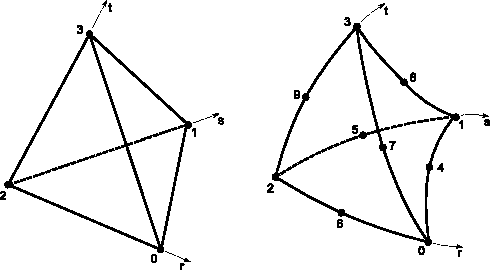
\includegraphics[width=8.5cm]{Figures/Tet4and10.pdf}
\caption{Linear tetrahedron with 4 nodes (tet4) and quadratic tetrahedron with 10 nodes (tet10)}
\label{Tet4AndTet10Illustration}
\end{figure}


The isoparametric 4-node tetrahedron interpolates the position linearly between the nodes (Fig. \ref{Tet4AndTet10Illustration}). Consequently, the stress is constant over the element and the element shows significant volumetric locking for nearly incompressible materials \cite{Belytschko2000}. In contrast, the 10-node tetrahedron interpolates positions with 2nd order polynomials and doesn't suffer from severe volume locking. Thus, in the realm of mechanical engineering it is well known that quadratic tetrahedra perform much better than linear tetrahedral meshes in many scenarios \cite{Cifuentes1992}. This is especially true for the simulation of incompressible objects.

Typically, the shape functions are defined in a local coordinate system $(r,s,t)$ and all element based operations such as calculating deformations, extracting rotations or numerical integration are performed in this local coordinate system. Polynomial functions (\emph{shape functions}) are used to map the local coordinates to the global coordinate system. If the polynomial degree of the shape functions matches the order of the basis functions, the element is called isoparametric. In case of the isoparametric 10-node tetrahedron, the shape functions are quadratic, which allows curved boundaries and therefore better approximation of the geometry (Fig. \ref{Tet4AndTet10Illustration}). 

As previously mentioned, the integrals that arise during the computation of the forces and the stiffness matrix are evaluated numerically. One cubature point per element is sufficient in order to integrate the stiffness matrix term eq. (\ref{CoRotStiffnessMatrix}) if linear basis functions are used. In contrast, four sample points are necessary to integrate the 10-node tetrahedron. Consequently, four rotation matrices have to be extracted per element for accurate integration. Alternatively, it is possible to extract just one rotation matrix per element by only using the four corner vertices in order to compute the deformation gradient. In this case the element matrix can be pre-computed and the numerical integration can be omitted, which reduces the computational costs by 75\%. This simplification will be referred to as the single rotation quadratic tetrahedron.


\subsection{Numerical validation}

Numerical simulation studies on a simple beam geometry are performed in order to compare the efficiency of the linear tetrahedral (tet4), the quadratic tetrahedral (tet10) as well as the single rotation quadratic tetrahedral (tet10SR) elements. In the first scenario, the beam deforms under gravity, while it is subjected to a twisting deformation pattern in the second scenario (Fig. \ref{BeamTwistAndGravity}). Incompressible material models (Poisson's ration $\nu=0.49$) are used throughout the study. The linear and the quadratic corotated FEM were implemented using the Simulation Open Framework Architecture (SOFA) toolkit \cite{Faure2012}. For all simulations in this study, the Newmark time integration scheme is used along with the Pardiso direct sparse solver from the Intel MKL 10.3.

\begin{figure}
   \centering   
   \psfragfig[width=0.98\textwidth]{Figures/BeamTwistAndGravity}
	\caption{Deformation under gravity (a) and twisting deformation pattern of a beam (b). A 1461 DOF tet4 mesh is compared to a 714 DOF tet10 mesh. The tet10SR element fails to capture the rotation at low resolution (b, middle), but achieves similar accuracy to the tet10 element at higher resolution (b, right).}
\label{BeamTwistAndGravity}
\end{figure}

In order to perform a quantitative analysis of the discretization error for each model, a reference solution on a high resolution quadratic mesh (100k elements) is computed for both problems. Test models of different resolutions are subsequently compared to this reference model.  We choose the root mean squared (RMS) error at the nodes of the reference solution as the error measures. The RMS errors with respect to the degrees of freedom (DOF) are depicted in Fig. \ref{ConvergenceQuadraticBeam}.

\begin{figure}
   \centering   
   \psfragfig[width=0.98\textwidth]{Figures/ConvergenceQuadraticBeam}
	\caption{RMS error over DOF for twisting deformation (left) and gravity induced deformation (right). The tet10 (green) and tet10SR (blue) elements show far superior accuracy for the same DOF than the tet4 (red) mesh.}
\label{ConvergenceQuadraticBeam}
\end{figure}

In case of the gravity induced deformation, tet4 elements need much more DOF (up to 40x) than tet10 elements in order to achieve the same accuracy. This result illustrates the locking behavior of linear tetrahedral elements. It should also be pointed out that the tet10SR formulation shows only negligible difference to the fully integrated tet10 element. Due to the displacement boundary conditions and the absence of volumetric forces, the difference in the twisting scenario is not as pronounced. However, the tet4 elements still need an order of magnitude more DOFs. It is apparent from Fig. \ref{BeamTwistAndGravity} that the tet4 mesh with 1461 DOFs still shows visible edges, while the lower resolution tet10 mesh (714 DOFs) produces a smooth deformation. It can also be seen that the tet10SR element fails to capture the rotations at low resolution (Fig. \ref{BeamTwistAndGravity}), but achieves a similar accuracy as the tet10 element for higher resolutions (right). It can be concluded that quadratic elements are superior to tet4 elements in both scenarios. Furthermore, the single rotation quadratic tetrahedral formulation (tet10SR) can be a computationally efficient alternative to the standard tet10 formulation for many applications.
